% IAM-UA8-F02 layout B (three panels, recommended): global mesh, structured region with the integration domain, symmetry detail.
% Preview at the printed size; not part of main_ua.tex.
% IAM-UA8-F02 preview preamble: the page geometry, fonts and caption settings of main_ua.tex (A4, 12 pt, margins 22 mm,
% text width 166 mm, STIX Two Text/Math, Ukrainian), so the previews show the figure at its intended printed size.
\documentclass[a4paper,12pt]{article}
\usepackage[margin=22mm]{geometry}
\usepackage{fontspec}
\usepackage{polyglossia}
\setdefaultlanguage{ukrainian}
\setotherlanguage{english}
\setmainfont{STIXTwoText-Regular.otf}[BoldFont=STIXTwoText-Bold.otf,ItalicFont=STIXTwoText-Italic.otf,BoldItalicFont=STIXTwoText-BoldItalic.otf]
\newfontfamily\cyrillicfont{STIXTwoText-Regular.otf}[Script=Cyrillic,Ligatures=TeX,BoldFont=STIXTwoText-Bold.otf,ItalicFont=STIXTwoText-Italic.otf,BoldItalicFont=STIXTwoText-BoldItalic.otf]
\usepackage{amsmath}
\usepackage{unicode-math}
\setmathfont{STIXTwoMath-Regular.otf}[Scale=1.0]
\usepackage{graphicx}
\usepackage{subcaption}
\captionsetup{font=small}
\captionsetup[subfigure]{font=small,skip=3pt,justification=raggedright}
\pagestyle{empty}
\graphicspath{{../../figures/iam_f02/}}

\begin{document}
\begin{figure}[t]
  \centering
  \begin{minipage}{\textwidth}
  \begin{subfigure}[t]{0.485\linewidth}
    \centering
    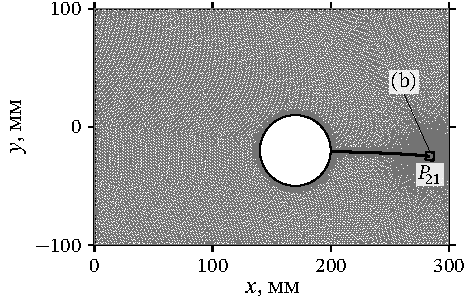
\includegraphics[width=\linewidth]{a_global_mesh.pdf}
    \caption{Сітка всієї пластини.}
  \end{subfigure}\hfill
  \begin{subfigure}[t]{0.485\linewidth}
    \centering
    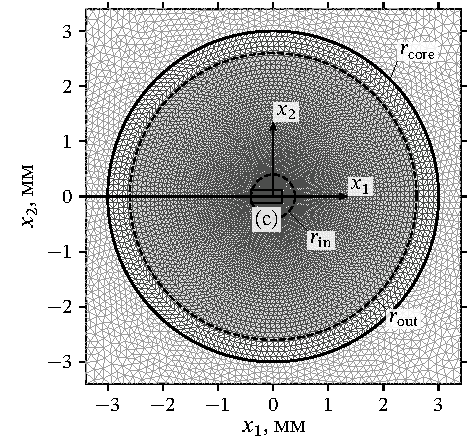
\includegraphics[width=\linewidth]{b_structured_region.pdf}
    \caption{Структурована привершинна область.}
  \end{subfigure}

  \vspace{4pt}
  \centering
  \begin{subfigure}[t]{0.94\linewidth}
    \centering
    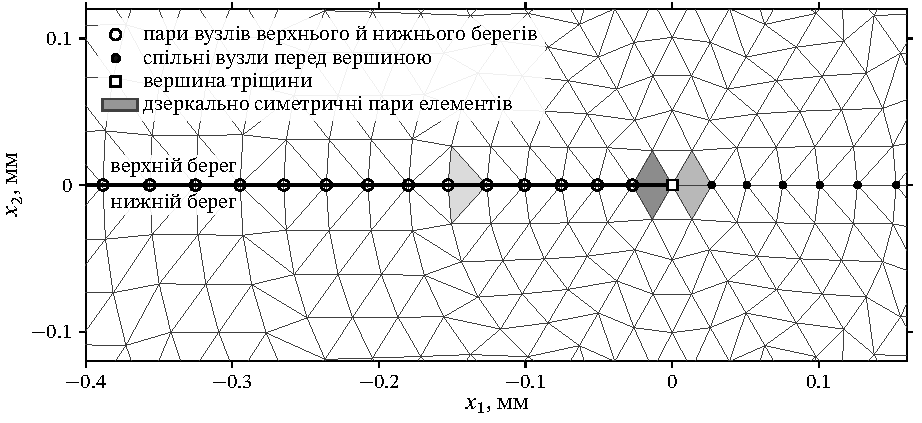
\includegraphics[width=\linewidth]{c_symmetry_detail.pdf}
    \caption{Дзеркальна симетрія сітки біля вершини.}
  \end{subfigure}
  \end{minipage}
  \caption{Скінченно-елементна сітка для прийнятого стану $P_{21}$ (${a=84}$~мм) траєкторії M0.
  (a)~Уся пластина з отвором, ламаною тріщиною та згущенням сітки біля поточної вершини; квадратом позначено область~(b).
  (b)~Структурована область радіуса ${r_{\mathrm{core}}=3}$~мм у локальній системі координат останньої ланки та перехід до
  неструктурованої зовнішньої сітки. Сірим виділено елементи, у яких вагова функція інтеграла взаємодії змінюється між
  ${r_{\mathrm{in}}=0.4}$~мм і ${r_{\mathrm{out}}=2.6}$~мм; прямокутником позначено область~(c).
  (c)~Фрагмент тієї самої сітки з кроком ${h_0=0.027012}$~мм: три пари дзеркально симетричних елементів, пари різних вузлів
  верхнього й нижнього берегів в одній точці та спільні вузли перемички перед вершиною.}
\end{figure}
\end{document}
